% !TeX spellcheck = russian-aot-ieyo
% Зачем: Определяет класс документа (То, как будет выглядеть документ)
% Примечание: параметр draft помечает строки, вышедшие за границы страницы, прямоугольником, в фильной версии его нужно удалить.
\documentclass[a4paper,14pt,russian,ukrainian,oneside,final]{extreport}

% Зачем: Установка кодировки исходных файлов.
\usepackage[utf8]{inputenc}

% Зачем: Делает результирующий PDF "searchable and copyable".
\usepackage{cmap}

% Зачем: Выбор внутренней TeX кодировки.
\usepackage[T2A]{fontenc}

% Зачем: Чтобы можно было использовать русские буквы в формулах, но в случае использования предупреждать об этом.
\usepackage[warn]{mathtext}

% Зачем: Учет особенностей различных языков.
\usepackage[russian]{babel}

% Зачем: Улучшает отображение русских шрифтов.
% Примечание: Требует шаманства при установке, инструкция http://plumbum-blog.blogspot.com/2010/06/miktex-28-pscyr-04d.html
%\usepackage{pscyr}


% Зачем: Добавляет поддержу дополнительных размеров текста 8pt, 9pt, 10pt, 11pt, 12pt, 14pt, 17pt, and 20pt.
% Почему: Пункт 2.1.1 Требований по оформлению пояснительной записки.
%\usepackage{extsizes}


% Зачем: Длинна, пимерно соответвующая 5 символам
% Почему: Требования содержат странное требование про отсупы в 5 символов (для немоноширинного шрифта :| )
\newlength{\fivecharsapprox}
\setlength{\fivecharsapprox}{6ex}
\newlength{\fivecharsapproxs}
\setlength{\fivecharsapproxs}{1ex}

% Зачем: Добавляет отступы для абзацев.
% Почему: Пункт 2.1.3 Требований по оформлению пояснительной записки.
\usepackage{indentfirst}
\setlength{\parindent}{\fivecharsapprox} % Примерно соответсвует 5 символам.


% Зачем: Настраивает отступы от границ страницы.
% Почему: Пункт 2.1.2 Требований по оформлению пояснительной записки.
\usepackage[left=3cm,top=2.0cm,right=1.5cm,bottom=2.7cm]{geometry}


% Зачем: Настраивает межстрочный интервал, для размещения 40 +/- 3 строки текста на странице.
% Почему: Пункт 2.1.1 Требований по оформлению пояснительной записки.
\usepackage[nodisplayskipstretch]{setspace} 
\setstretch{1.1}
%\onehalfspacing

% Зачем: Выбор шрифта по-умолчанию. 
% Почему: Пункт 2.1.1 Требований по оформлению пояснительной записки.
% Примечание: В требованиях не указан, какой именно шрифт использовать. По традиции используем TNR.
\renewcommand{\rmdefault}{ftm} % Times New Roman


% Зачем: Отключает использование изменяемых межсловных пробелов.
% Почему: Так не принято делать в текстах на русском языке.
\frenchspacing


% Зачем: Сброс счетчика сносок для каждой страницы
% Примечание: в "Требованиях по оформлению пояснительной записки" не указано, как нужно делать, но в других БГУИРовских докуметах рекомендуется нумерация отдельная для каждой страницы
\usepackage{perpage}
\MakePerPage{footnote}


% Зачем: Добавляет скобку 1) к номеру сноски
% Почему: Пункты 2.9.2 и 2.9.1 Требований по оформлению пояснительной записки.
\makeatletter 
\def\@makefnmark{\hbox{\@textsuperscript{\normalfont\@thefnmark)}}}
\makeatother


% Зачем: Расположение сносок внизу страницы
% Почему: Пункт 2.9.2 Требований по оформлению пояснительной записки.
\usepackage[bottom]{footmisc}


% Зачем: Переопределяем стандартную нумерацию, т.к. в отчете будут только section и т.д. в терминологии TeX
\makeatletter
\renewcommand{\thesection}{ \arabic{section}}




\makeatother


% Зачем: Пункты (в терминологии требований) в терминологии TeX subsubsection должны нумероваться
% Почему: Пункт 2.2.3 Требований по оформлению пояснительной записки.
\setcounter{secnumdepth}{3}


% Зачем: Настраивает отступ между таблицей с содержанимем и словом СОДЕРЖАНИЕ
% Почему: Пункт 2.2.7 Требований по оформлению пояснительной записки.
\usepackage{tocloft}
\setlength{\cftbeforetoctitleskip}{-1em}
\setlength{\cftaftertoctitleskip}{1em}





\usepackage{fancyhdr}
\pagestyle{fancy}
\fancyhf{}
\fancyhead[R]{\thepage}
\fancyheadoffset{0mm}
\fancyfootoffset{0mm}
\setlength{\headheight}{17pt}
\renewcommand{\headrulewidth}{0pt}
\renewcommand{\footrulewidth}{0pt}
\fancypagestyle{plain}{ 
    \fancyhf{}
    \rhead{\thepage}}

% Зачем: Определяет отступы слева для записей в таблице содержания.
% Почему: Пункт 2.2.7 Требований по оформлению пояснительной записки.
\makeatletter
\renewcommand{\l@section}{\@dottedtocline{1}{0.5em}{1.2em}}
\renewcommand{\l@subsection}{\@dottedtocline{2}{1.7em}{2.0em}}
\makeatother

% Зачем: Задает стиль заголовков раздела жирным шрифтом, прописными буквами, без точки в конце
% Почему: Пункты 2.1.1, 2.2.5, 2.2.6 и ПРИЛОЖЕНИЕ Л Требований по оформлению пояснительной записки.
\makeatletter
\renewcommand\section{%
  \clearpage\@startsection {section}{0}%
    {\fivecharsapproxs}%
    {-1em \@plus -1ex \@minus -.2ex}%
    {1em \@plus .2ex}%
    {\raggedright\hyphenpenalty=10000\normalfont\large\bfseries\MakeUppercase {}}
}
\makeatother


% Зачем: Задает стиль заголовков подразделов
% Почему: Пункты 2.1.1, 2.2.5 и ПРИЛОЖЕНИЕ Л Требований по оформлению пояснительной записки.
\makeatletter
\renewcommand\subsection{%
  \@startsection{subsection}{2}%
    {\fivecharsapprox}%
    {-1em \@plus -1ex \@minus -.2ex}%
    {1em \@plus .2ex}%
    {\raggedright\hyphenpenalty=10000\normalfont\normalsize\bfseries}}
\makeatother


% Зачем: Задает стиль заголовков пунктов
% Почему: Пункты 2.1.1, 2.2.5 и ПРИЛОЖЕНИЕ Л Требований по оформлению пояснительной записки.
\makeatletter
\renewcommand\subsubsection{
  \@startsection{subsubsection}{3}%
    {\fivecharsapprox}%
    {-1em \@plus -1ex \@minus -.2ex}%
    {\z@}%
    {\raggedright\hyphenpenalty=10000\normalfont\normalsize\bfseries}}
\makeatother

% Зачем: для оформления введения и заключения, они должны быть выровнены по центру.
% Почему: Пункты 1.1.15 и 1.1.11 Требований по оформлению пояснительной записки.
\makeatletter
\newcommand\sectioncentered{%
  \clearpage\@startsection {section}{1}%
    {\z@}%
    {-1em \@plus -1ex \@minus -.2ex}%
    {1em \@plus .2ex}%
    {\centering\hyphenpenalty=10000\normalfont\large\bfseries\MakeUppercase}%
    }
\makeatother



% Зачем: Задает стиль библиографии
% Почему: Пункт 2.8.6 Требований по оформлению пояснительной записки.
\bibliographystyle{styles/belarus-specific-utf8gost780u}


% Зачем: Пакет для вставки картинок
% Примечание: Объяснение, зачем final - http://tex.stackexchange.com/questions/11004/why-does-the-image-not-appear
\usepackage[final]{graphicx}
\DeclareGraphicsExtensions{.pdf,.png,.jpg,.eps}


% Зачем: Директория в которой будет происходить поиск картинок
\graphicspath{{figures/}}


% Зачем: Добавление подписей к рисункам
\usepackage[nooneline]{caption}
\usepackage{subcaption}

% Зачем: Задание подписей, разделителя и нумерации частей рисунков
% Почему: Пункт 2.5.5 Требований по оформлению пояснительной записки.
\DeclareCaptionLabelFormat{stbfigure}{Рис. #2}
\DeclareCaptionLabelFormat{stbtable}{Таблица #2}
\DeclareCaptionLabelSeparator{stb}{~~}
\captionsetup{labelsep=stb}
\captionsetup[figure]{labelformat=stbfigure,justification=centering}
\captionsetup[table]{labelformat=stbtable,justification=raggedright}
\renewcommand{\thesubfigure}{\asbuk{subfigure}}

% Зачем: Окружения для оформления формул
% Почему: Пункт 2.4.7 требований по оформлению пояснительной записки и специфические требования различных кафедр
\usepackage{tabularx}

\newenvironment{explanation}
    {
    %%% Следующие строки определяют специфические требования кафедр. Раскоменнтируйте нужные 2 строки
    %% стандартный абзац, Кафедра информатики
    \par 
    \tabularx{\textwidth-\fivecharsapprox}{@{}ll@{ --- } X }
    %% без отступа, Кафедра экономической информатики
    %\noindent 
    %\tabularx{\textwidth}{@{}ll@{ --- } X }
    }
    { 
    \\[\parsep]
    \endtabularx
    }


% Зачем: Удобная вёрстка многострочных формул, масштабирующийся текст в формулах, формулы в рамках и др
\usepackage{amsmath}


% Зачем: Поддержка ажурного и готического шрифтов 
\usepackage{amsfonts}


% Зачем: amsfonts + несколько сотен дополнительных математических символов
\usepackage{amssymb}


% Зачем: Окружения «теорема», «лемма»
\usepackage{amsthm}


% Зачем: Производить арифметические операции во время компиляции TeX файла
\usepackage{calc}

% Зачем: Производить арифметические операции во время компиляции TeX файла
\usepackage{fp}

% Зачем: Пакет для работы с перечислениями
\usepackage{enumitem}
\makeatletter
 \AddEnumerateCounter{\asbuk}{\@asbuk}{щ)}
\makeatother


% Зачем: Устанавливает символ начала простого перечисления
% Почему: Пункт 2.3.5 Требований по оформлению пояснительной записки.
\setlist{nolistsep}


% Зачем: Устанавливает символ начала именованного перечисления
% Почему: Пункт 2.3.8 Требований по оформлению пояснительной записки.
\renewcommand{\labelenumi}{\asbuk{enumi})}
\renewcommand{\labelenumii}{\arabic{enumii})}

% Зачем: Устанавливает отступ от границы документа до символа списка, чтобы этот отступ равнялся отступу параграфа
% Почему: Пункт 2.3.5 Требований по оформлению пояснительной записки.

\setlist[itemize,0]{itemindent=\parindent + 2.2ex,leftmargin=0ex,label=--}
\setlist[enumerate,1]{itemindent=\parindent + 2.7ex,leftmargin=0ex}
\setlist[enumerate,2]{itemindent=\parindent + \parindent - 2.7ex}

% Зачем: Включение номера раздела в номер формулы. Нумерация формул внутри раздела.
\AtBeginDocument{\numberwithin{equation}{section}}

% Зачем: Включение номера раздела в номер таблицы. Нумерация таблиц внутри раздела.
\AtBeginDocument{\numberwithin{table}{section}}

% Зачем: Включение номера раздела в номер рисунка. Нумерация рисунков внутри раздела.
\AtBeginDocument{\numberwithin{figure}{section}}


% Зачем: Дополнительные возможности в форматировании таблиц
\usepackage{makecell}
\usepackage{multirow}
\usepackage{array}


% Зачем: "Умная" запятая в математических формулах. В дробных числах не добавляет пробел
% Почему: В требованиях не нашел, но в русском языке для дробных чисел используется {,} а не {.}
\usepackage{icomma}

% Зачем: макрос для печати римских чисел
\makeatletter
\newcommand{\rmnum}[1]{\romannumeral #1}
\newcommand{\Rmnum}[1]{\expandafter\@slowromancap\romannumeral #1@}
\makeatother


% Зачем: Управление выводом чисел.
\usepackage{sistyle}
\SIdecimalsign{,}

% Зачем: inline-коментирование содержимого.
\newcommand{\ignore}[2]{\hspace{0in}#2}


% Зачем: Возможность коментировать большие участки документа
\usepackage{verbatim}


\usepackage{xcolor}


% Зачем: Оформление листингов кода
% Примечание: final нужен для переопределения режима draft, в котором листинги не выводятся в документ.
\usepackage[final]{listings}


% Зачем: настройка оформления листинга для языка F#
\definecolor{bluekeywords}{rgb}{0.13,0.13,1}
\definecolor{greencomments}{rgb}{0,0.5,0}
\definecolor{turqusnumbers}{rgb}{0.17,0.57,0.69}
\definecolor{redstrings}{rgb}{0.5,0,0}

\renewcommand{\lstlistingname}{Листинг}

\lstdefinelanguage{FSharp}
    {morekeywords={abstract,and,as,assert,base,begin,class,default,delegate,do,done,downcast,downto,elif,else,end,exception,extern,false,finally,for,fun,function,global,if,in,inherit,inline,interface,internal,lazy,let,let!,match,member,module,mutable,namespace,new,not,null,of,open,or,override,private,public,rec,return,return!,select,static,struct,then,to,true,try,type,upcast,use,use!,val,void,when,while,with,yield,yield!,asr,land,lor,lsl,lsr,lxor,mod,sig,atomic,break,checked,component,const,constraint,constructor,continue,eager,event,external,fixed,functor,include,method,mixin,object,parallel,process,protected,pure,sealed,tailcall,trait,virtual,volatile},
    keywordstyle=\bfseries\color{bluekeywords},
    sensitive=false,
    morecomment=[l][\color{greencomments}]{///},
    morecomment=[l][\color{greencomments}]{//},
    morecomment=[s][\color{greencomments}]{{(*}{*)}},
    morestring=[b]",
    stringstyle=\color{redstrings},
    }

\lstdefinestyle{fsharpstyle}{
   xleftmargin=0ex,
   language=FSharp,
   basicstyle=\footnotesize\ttfamily,
   breaklines=true,
   columns=fullflexible
}

\lstdefinestyle{csharpinlinestyle} {
  language=[Sharp]C,
  morekeywords={yield,var,get,set,from,select,partial,where,async,await},
  breaklines=true,
  columns=fullflexible,
  basicstyle=\footnotesize\ttfamily
}

\lstdefinestyle{csharpstyle}{
  language=[Sharp]C,
  frame=lr,
  rulecolor=\color{blue!80!black}}


% Зачем: Нумерация листингов в пределах секции
\AtBeginDocument{\numberwithin{lstlisting}{section}}

\usepackage[normalem]{ulem}

\usepackage[final,hidelinks]{hyperref}
% Моноширинный шрифт выглядит визуально больше, чем пропорциональный шрифт, если их размеры одинаковы. Искусственно уменьшаем размер ссылок.
\renewcommand{\UrlFont}{\small\rmfamily\tt}

\usepackage[square,numbers,sort&compress]{natbib}
\setlength{\bibsep}{0em}

% Магия для подсчета разнообразных объектов в документе
\usepackage{lastpage}
\usepackage{totcount}
\regtotcounter{section}

\usepackage{etoolbox}

\newcounter{totfigures}
\newcounter{tottables}
\newcounter{totreferences}
\newcounter{totequation}

\providecommand\totfig{} 
\providecommand\tottab{}
\providecommand\totref{}
\providecommand\toteq{}

\makeatletter
\AtEndDocument{%
  \addtocounter{totfigures}{\value{figure}}%
  \addtocounter{tottables}{\value{table}}%
  \addtocounter{totequation}{\value{equation}}
  \immediate\write\@mainaux{%
    \string\gdef\string\totfig{\number\value{totfigures}}%
    \string\gdef\string\tottab{\number\value{tottables}}%
    \string\gdef\string\totref{\number\value{totreferences}}%
    \string\gdef\string\toteq{\number\value{totequation}}%
  }%
}
\makeatother

\pretocmd{\section}{\addtocounter{totfigures}{\value{figure}}\setcounter{figure}{0}}{}{}
\pretocmd{\section}{\addtocounter{tottables}{\value{table}}\setcounter{table}{0}}{}{}
\pretocmd{\section}{\addtocounter{totequation}{\value{equation}}\setcounter{equation}{0}}{}{}
\pretocmd{\bibitem}{\addtocounter{totreferences}{1}}{}{}



% Для оформления таблиц не влязящих на 1 страницу
\usepackage{longtable}

% Для включения pdf документов в результирующий файл
\usepackage{pdfpages}

% Зачем: Переносы в словах с тире.
% Тире в словае заменяем на \hyph: аппаратно\hyphпрограммный.
% https://stackoverflow.com/questions/2193307/how-to-get-latex-to-hyphenate-a-word-that-contains-a-dash#
\def\hyph{-\penalty0\hskip0pt\relax}

\usepackage{rotating}
%%%%%%%%%%%%%%%%%%%%%%%%%%%%%%%%%%%%%%%%%%%
%%%%%%%%%%%%%%%%%%%%%%%%%%%%%%%%%%%%%%%%%%%
%%%%%%%%%%%%%%%%%%%%%%%%%%%%%%%%%%%%%%%%%%%
%%%%%%%%%%%%%%%%%%%%%%%%%%%%%%%%%%%%%%%%%%%
\begin{document}
\setcounter{page}{2}
\renewcommand \contentsname {\centerline{\bfseries\large{\MakeUppercase{Зміст}}}}

% Зачем: Не захламлять основной файл
% Примечание: \small\selectfont злостный хак, чтобы уменьшить размер шрифта в ToC 
{

\normalsize\selectfont
\tableofcontents
\newpage
}

\setlength{\parindent}{1.25cm}
\sectioncentered*{Вступ}
\addcontentsline{toc}{section}{Вступ}
\label{sec:intro}

\indent Орієнтовану мережу можна інтерпретувати як деяку транспортну мережу і використовувати її для вирішення задач про потоки речовин в системі трубопроводів. Уявімо, що деякий продукт передається по системі від джерела, де даний продукт виробляється, до стоку, де він споживається. 
Джерело виробляє продукт з деякою максимальною швидкістю, а стік з тією ж швидкістю споживає продукт. Потоком продукту в будь-якій точці системи є швидкість руху продукту.
За допомогою транспортних мереж можна моделювати течію рідин
по трубопроводах, рух деталей на складальних лініях, передачу струму по
електричним мережам, інформації - в інформаційних мереж і т. д. Кожне
орієнтоване ребро мережі можна розглядати як канал, по якому рухається продукт. Кожен канал має задану пропускну здатність, яка характеризує максимальну швидкість переміщення продукту по каналу.
Вершини є точками перетину каналів. Через вершини, відмінні від
джерела і стоку, продукт проходить не накопичуючись.

У задачі про максимальний потік ми хочемо знайти максимальну швидкість
пересилання продукту від джерела до стоку, при якій не будуть порушуватися
обмеження пропускної здатності. Ця проблема була поставлена Т.Є. Харрісом навесні 1955 року, який разом з відставним генералом Ф.С. Россом запропонував спрощену модель залізничного транспортного потоку і висунув саме цю спеціальну задачу як центральну, підказаною цією моделлю. Незабаром після цього був висловлений в якості гіпотези, а потім і встановлений головний результат - теорема «Про максимальний потік і мінімальний розріз».
\par{}У даній роботі розглядається узагальнений метод Форда-Фалкерсона для транспортної мережі з обмеженою пропускною здатністю дуг а також з ціною за транспортування одиниці продукту через мережу. В якості алгоритму побудови рішення був обраний алгоритм Баскера-Гоуєна.

\section{ Задача про максимальний потік }
\subsection{Постановка задачі}

\indent{\it Орієнтованої мережею } 
називається граф $G = [V, E]$, який складається із сукупності $V$ елементів $x, y, ...$ разом з множиною $E$ деяких впорядкованих пар $(x, y)$ елементів, взятих з $V$.

{\it Вузли} - елементи множини $V$.
	
{\it Дуги} - елементи множини $E$. Можливість дуги $(x,x)$ вилучається.

Поставимо кожній дузі $(x, y)$ у відповідність деяке число $c (x, y)$ ,яке називається пропускною здатністю дуги. Пропускна здатність показує яка кількість речовини може пройти по цій дузі в одиницю часу. 

Потоком (flow) в мережі є дійсна функція $f: VxV-> R$ задовольняє трьом умовам:
\begin{enumerate}
\item обмеження пропускної здатності $$\forall u,v \in V f(u,v)\leqslant c(u,v)$$
Потік з однієї вершини в іншу не повинен перевищувати задану пропускну здатність.
\item антисиметричність $$f(u,v)=-f(v,u) \forall u,v \in V$$
Потік з вершини $u$ в вершину $v$ протилежний потоку у зворотному напрямку.
\item збереження потоку $$\forall u \in V/s,t \sum_{v\in V} f(u,v)=0$$
\end{enumerate}
Сумарний потік, що виходить з вершини, що не є джерелом або стоком дорівнює нулю. Величина потоку визначається як сумарний потік, що виходить з джерела.
$$|f|=\sum_{v\in V}f(s,v)$$
Будемо називати $s$ {\it джерелом} $t$ {\it стоком}, а інші вузли - проміжними.

Задача про максимальний потік (maximum flow poblem) полягає в знаходженні потоку максимальної величини. Математично постановка виглядає так:
$$
\begin{aligned}
&max\quad  v=f(s,V)& \\
&f(x,V)-f(V,X)=0, &x\neq s,t, \\
&0\leqslant f(x,y) \leqslant c(x,y) , &(x,y)\in E,
\end{aligned} 
$$

\subsection{Метод Форда-Фалкерсона}
Метод Форда-Фалкерсона базується на трьох важливих концепціях. Це залишкові мережі, що збільшують шляхи і розрізи. 
Метод є ітеративним. Спочатку значення потоку  встановлюється нуль. $f(u,v)=0  \forall u,v \in V$ На кожній ітерації величина потоку збільшується 
за допомогою пошуку збільшуючого шляху (деякого шляху від джерела до стоку вздовж якого можна відправити більший потік) і подальшого збільшення потоку. 
Цей процес повторюється до тих пір, поки вже неможливо відшукати збільшуваного шлях.

\indent Залишкові мережі

\indent Нехай задана транспортна мережа $G(V,E)$ з джерелом $s$ і стоком $t$. Нехай $f$ деякий потік в $G$.
Розглянемо пару вершин $u,v \in V$. Величина додаткового потоку, який ми можемо 
направити з $u$ в $v$, щоб не перевищити пропускну здатність $c(u,v)$ є залишковою 
пропускною здатністю ребра $(u,v)$ і задається формулою:
$$c_{f}(u,v)=c(u,v)-f(u,v)$$

Для транспортної $G(V,E)$ мережі і потоку $f$ залишковою мережею в $G$, породженою потоком $f$ є мережа 
$G_{f}=(V,E_{f})$  где $$E_{f}=(u,v)\in VxV:c_{f}(u,v)>0$$
Таким чином по кожному ребру залишкової мережі або залишковому ребру можна направити потік більше нуля.

\indent Збільшуючі шляхи

\indent Для заданої транспортної мережі $G=(V,E)$ і потоку $f$ збільшуючим шляхом $p$ є простий шлях з $s$ в $t$ в залишковій мережі $G_{f}$.
Максимальна величина, на яку можна збільшити потік уздовж кожного ребра $p$ збільшуючого шляху називається пропускною здатністю шляху і задається формулою:
$$c_{f}(p)=min\{c(u,v):(u,v)\in p\}$$.

\indent Розрізи транспортних мереж

\indent Розрізом транспортної мережі $G(V,E)$ називається розбиття множини вершин на множини $S$ та $T$ такі що $s\in S, t\in T$.
Якщо $f$ потік - то чистий потік через розріз $(S,T)$ визначимо як $f(S,T)$.
Пропускну здатність розрізу $(S,T)$ визначимо відповідно $c(S,T)$.
Мінімальним розрізом є розріз, пропускна здатність якого серед всіх розрізів мінімальна. Як видно, 
потік через розріз, на відміну від пропускної здатності розрізу, може включати і від’ємні доданки.
\newtheorem{theorem}{Теорема}
\begin{theorem}[ Про максимальний потік і мінімальний розріз]
Для будь-якої мережі максимальна величина потоку з $s$ в $t$ 
дорівнює мінімальній пропускній здатності розрізу, що відокремлює $s$ и $t$.  \cite{ford}
\end{theorem}


\section{ Задача про максимальний потік мінімальної вартості}
\subsection{Постановка задачі}
Нехай, кожній дузі відповідає не лише пропускна здатність, а також і велечина $c_{ij}>0$ яка дорівнює вартості транспортування одиниці товару через ребро $(i,j)\in E$ мережі.
Задача пошука потока  із $s$ в $t$ заданої потужності $v$  і мінімальної вартості має вигляд:
$$Z=\sum_{(i,j)\in E} c_{ij}x_{ij}\to min_{x};$$
$$\sum_{i:(i,j)\in E}x_{ij}-\sum_{k:(j,k)\in E}x_{jk}=
 \begin{cases}
   -v, &j=s;\\
   0, &j \neq s,t;\\
   v,&j=t;
 \end{cases}$$
$$
0\leq x_{ij}\leq b_{ij}, (i,j)\in E
$$

 

\subsection{Алгоритм Баскера-Гоуєна}
Для розв'язування задачі про максимальний потік мінімальної вартостіі будемо використовувати алгоритм Баскера-Гоуєна:
\begin{enumerate}
\item Знайдемо поток мінімальної вартості із $ s $ в $ t $.
\item З'ясуемо максимальну величину потоку, яку можна пропустити через цей шлях.
\item Якщо ця велечина більша за потрібну потужність мережі, візмемо її рівною потрібній потужності.
\item 	Збільшити поток по цьому потоку на максимальну величину(але так щоб загальний  поток через мережу не перевищував потрібний)
\item 	Розрахувати ціну за транспортування потужності. Додати до загальної ціни потоку.
\item 	Якщо поток по мережі дорівнюе заданому, то припинити роботу алгоритму. Інакше перейти на крок $a$ з оновленими велечинами потоків.
\end{enumerate}

\subsection{Програмна реалізація}

В програмній реалізації пошук потоку мінімальної вартості виглядає наступним чином:

\indent Починаючи з джерела кожна вершина пов'язана з данною додаеться до черги (queue). При цьому для вершини запам'ятовується  вершина, з якої ми до неї прийшли, та загальа вартість потоку по цьому шляху. Для того щоб порахувати загальну вартість потоку треба  знайти мінімальну пропускну здатність шляху, а потім знайти сумму добутків мінімальної пропускної здатності шляху на ціну на кожній дузі шляху.

\indent В результаті на $n$-му кроці алгоритму ми прийдемо до стоку $t$ і при цьому будемо знати яку величину потоку ми можео пропустити по шляху і його повну вартість. Якщо вершина вже була оброблена алгоритмом і для неї ми знаємо суммарну вартість і батьківську вершину то батьківською оберається та вершина яка дає меншу суммарну  ціну за транспортування.

\indent Будемо виконувати алгоритм доки в черзі є хоч один елемент. Якщо елементи в черзі закінчилися то перевіримо чи є у вершини-стоку $t$ батькывська вершина. Якщо так то ми можемо дізнатися велечину потока по цьому шляху, його вартість, а також вершини і ребра, що є елементами цього шляху. Перерахуємо повну пропускну здатність мережі та вартість потоку по ній. Використаемо ці данні для того щоб перерахувати пропускну здатність мережі і перейдемо на перший крок алгоритму з новими данними. Якщо ні, тоді шляху з джерела в сток немає. Максимальна пропускна здатність і ціна дорівнюють останнім розрахованим велечинам.

\indent Программа виконана у вигляді додатку для командної строки на мові програмування c\#.
Для запуску программи треба виконати програму передавши їй назву файла (без формату) як перший агрумент. Программа зчитує данні з файлу у форматі .csv (данні розділені запятою).
Наприклад якщо початкові данні лежать у файлі main.csv то у вікні командної строки треба виконати наступну команду:

$$MinCostFlow.exe \quad main$$

Після закінчення роботи програми результат буде записано в файл з такою ж назвою як і файл з початковими данними і текстом \_result у кінці назви.
Користувач побачить провідомлення про це англійською мовою.
В разі аварійної зупинки програми користувач дізнаетья про це за текстом помилки на екрані (наприклад якщо файла з таким ім'ям немає).

Також була протестована швидкість роботи программи. Для цього я згенерував повний граф (кожна вершина пов'язана з усіма іншими) з тисячею вершин і випадковою пропускною здатністю вузлів (від 0 до 1000).
Таким ж чинов я згенерував матрицю вартостей транспортування.
Я хотів знайти мінімальну вартість максимально можливого потоку по цій мережі.
Як максимальний поток я обрав велечину яку отримав складанням пропускних здатностей всіх вершин, які йдуть до стоку.
Тобто граф мав $1000*1000=1000000$ ребер.
Час роботи программи склав приблизно 25 хвилин.


\section{Приклади}
Задача 1

\indent У деякої компанії "Аврора" є фабрика в Берліні, що виробляє стільці, а в Бремені склад, де вони зберігаються. Компанія орендує місце на вантажівках інших фірм для доставки стільців з фабрики на склад. Оскільки вантажівки їздять по певних маршрутах між містами і мають обмежену вантажопідйомність, компанія може перевозити не більше певної кількості ящиків на день між містами. Також, компанія сплачує певну ціну за перевезення одиниці товару по кожному відсіку маршруту. Компанія не може вплинути на маршрути і пропускну здатність. Її завдання визначити, якими будуть витрати на перевезення 100 ящиків з Берліна до Бремена.

\indent Фабрику будемо вважати джерелом $(s)$, склад - стоком $(t)$. \\
Маршрути між містами будемо вважати ребрами мережі.\\
Вантажопідйомність вантажівок будемо вважати обмеженням пропускної спроможності на ребрах $c(u,v)$.
ціну за перевезення однієї коробки будемо вважати ціною ребра мережі $c_{ij}(v)$.
Занесемо дані в таблицю, де кожен елемент - обмеження пропускної здатності між відповідними містами (нуль означає що маршрут відсутній):
\begin{figure}[h]
\begin{center}
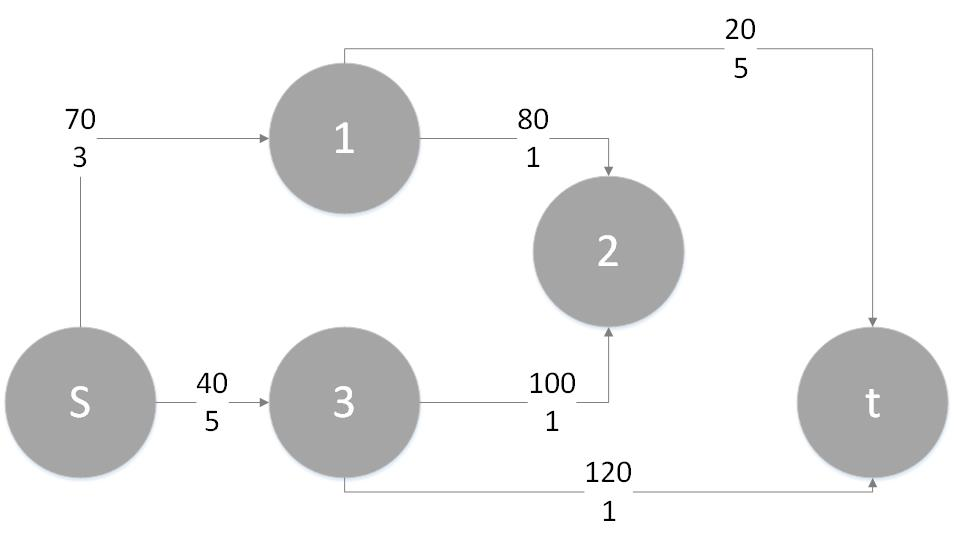
\includegraphics[scale=0.65]{G1.jpg}
\caption{Транспортна мережа}
\end{center}
\end{figure}
\\
\begin{center}
\begin{tabular}{|c|c|c|c|c|}
\hline
0&70&0&40&0 \\
\hline
0&0&80&0&20 \\
\hline
0&0&0&100&0 \\
\hline
0&0&0&0&120 \\
\hline
0&0&0&0&0 \\
\hline
\end{tabular}
\end{center}
Ціна за транспортування одиниці товару представмо у вигляді таблиці, де коже елемент - ціна за транспортування одиниці товару між містами:
\begin{center}
\begin{tabular}{|c|c|c|c|c|}
\hline
0&3&0&5&0 \\
\hline
0&0&1&0&5 \\
\hline
0&0&0&1&0 \\
\hline
0&0&0&0&1 \\
\hline
0&0&0&0&0 \\
\hline
\end{tabular}
\end{center}

\indent В результаті роботи програми було отримано наступне рішення:
\begin{center}
\begin{tabular}{|c|c|c|c|c|}
\hline
0&60&0&40&0 \\
\hline
0&0&60&0&0 \\
\hline
0&0&0&60&0 \\
\hline
0&0&0&0&100\\
\hline
0&0&0&0&0 \\
\hline
\end{tabular} \\
\begin{figure}[h]

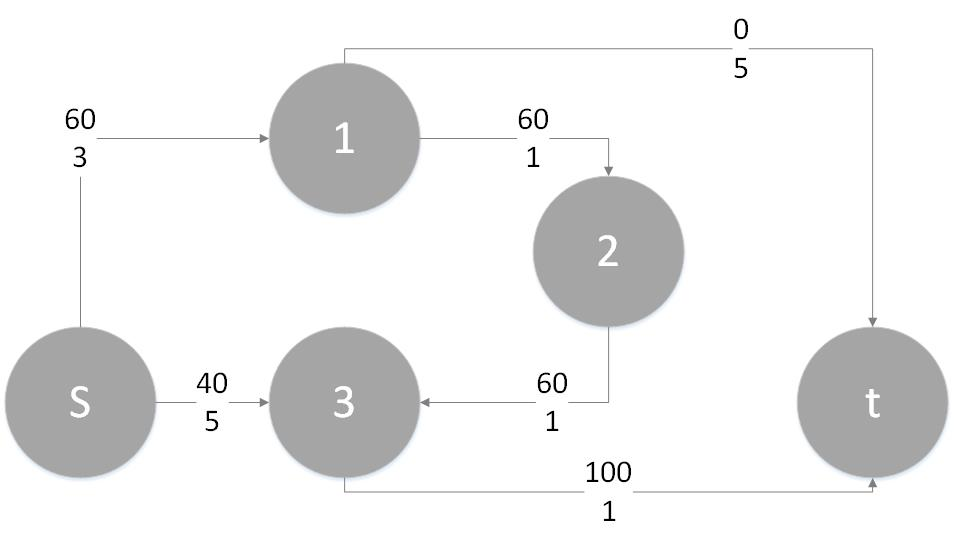
\includegraphics[scale=0.65]{G1_1.jpg}
\caption{Результуюча транспортна мережа}

\end{figure}
Повна вартість транспортування ста одиниць товару через мережу - 600 одиниць.
\end{center}


%%%%%%%%%%%%%%%%%%%%%%%%%%%%%%%%%%%%%%%%%%

Задача 2

\indent
Компанія постачальник високошвидкісного інтернету "Byte" отримала потенціального замовника, якому необхідно раз на день синхронізувати основну та запасну бази данних. Очікуваний розмір пакета данних 100 гігабайт. Постачальник послуг високошвидкісного інтернету знає пропускну здатність всіх вузлів своеї мережі, та вартість передачі одного гігабайту трафіку через кожне сполучення в мережі. "Byte" мінімізує свої витрати на синхронізацію. Їй треба знайти, яким шляхом маршрутизовати трафік та розрахувати мінімальну ціну, яку їй доведеться заплатити за передачу цих данних.

\indent
Зведемо дану задачу до задачі про максимальний потік.
\par Будемо вважати основний сервер джерелом $s$ а запасний стоком $t$. проміжні сполучення будемо вважати ребрами мережі, з обмеженнями на пропускну здатність $c(x,y)$ заданої в вигляді таблиці.
 Вартість передачі одного гігабайту будемо вважати ціною за транспортування $c_{ij}(v)$
\begin{figure}[h]
\begin{center}
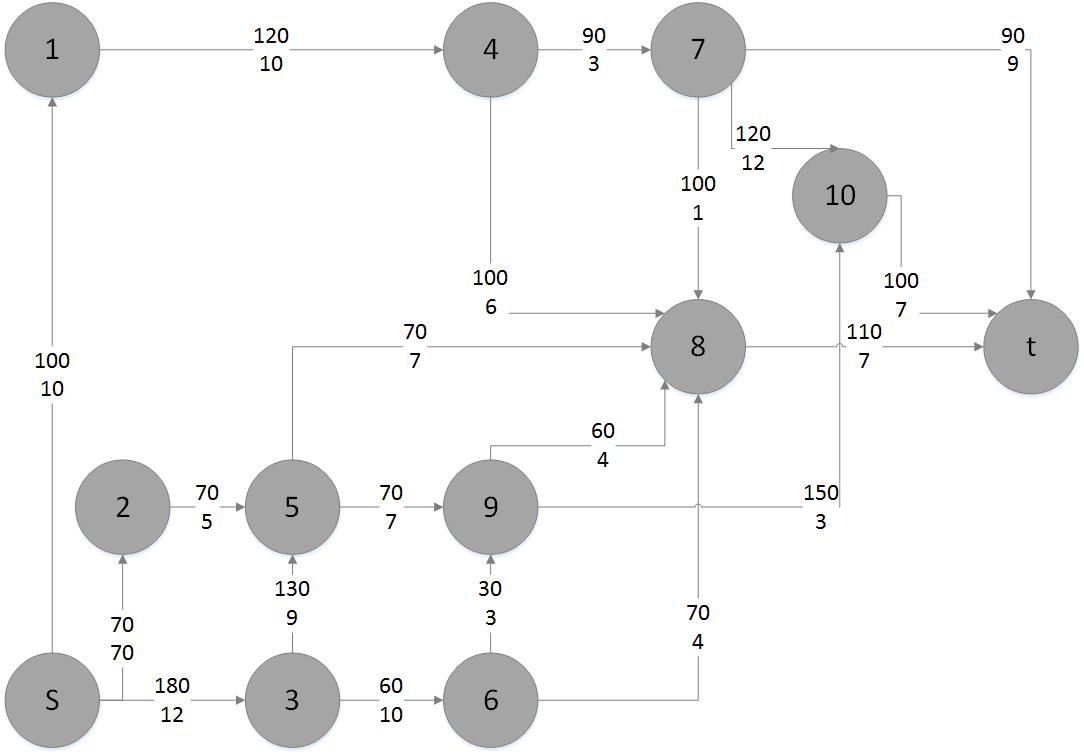
\includegraphics[scale=0.60]{G2.jpg}
\caption{Транспортна мережа}
\end{center}
\end{figure}
\\
\begin{center}
\begin{tabular}{|c|c|c|c|c|c|c|c|c|c|c|c|}
\hline
0&100&70&180&0&0&0&0&0&0&0&0 \\ \hline
0&0&0&0&120&0&0&0&0&0&0&0 \\ \hline
0&0&0&0&0&70&0&0&0&0&0&0 \\ \hline
0&0&0&0&0&130&60&0&0&0&0&0 \\ \hline
0&0&0&0&0&0&0&90&100&0&0&0 \\ \hline
0&0&0&0&0&0&0&0&70&70&0&0 \\ \hline
0&0&0&0&0&0&0&0&70&30&0&0 \\ \hline
0&0&0&0&0&0&0&0&100&0&120&90 \\ \hline
0&0&0&0&0&0&0&0&0&0&0&110 \\ \hline
0&0&0&0&0&0&0&0&60&0&150&0 \\ \hline
0&0&0&0&0&0&0&0&0&0&0&100 \\ \hline
0&0&0&0&0&0&0&0&0&0&0&0 \\ \hline
\end{tabular}
\end{center}
Вартість передачі одного гігабайту данних по проміжному ребру мережі задана таблицею.
\begin{center}
\begin{tabular}{|c|c|c|c|c|c|c|c|c|c|c|c|}
\hline
0&10&70&12&0&0&0&0&0&0&0&0\\ \hline
0&0&0&0&10&0&0&0&0&0&0&0  \\ \hline
0&0&0&0&0&5&0&0&0&0&0&0   \\ \hline
0&0&0&0&0&9&10&0&0&0&0&0  \\ \hline
0&0&0&0&0&0&0&3&6&0&0&0   \\ \hline
0&0&0&0&0&0&0&0&7&7&0&0   \\ \hline
0&0&0&0&0&0&0&0&4&3&0&0   \\ \hline
0&0&0&0&0&0&0&0&1&0&12&9  \\ \hline
0&0&0&0&0&0&0&0&0&0&0&7   \\ \hline
0&0&0&0&0&0&0&0&4&0&3&0   \\ \hline
0&0&0&0&0&0&0&0&0&0&0&7   \\ \hline
0&0&0&0&0&0&0&0&0&0&0&0   \\ \hline
\end{tabular}
\end{center}

\indent В результаті роботи програми було отримано наступне рішення:
\begin{center}
\begin{tabular}{|c|c|c|c|c|c|c|c|c|c|c|c|}
\hline
0&100&0&0&0&0&0&0&0&0&0&0 \\ \hline
0&0&0&0&100&0&0&0&0&0&0&0 \\ \hline
0&0&0&0&0&0&0&0&0&0&0&0   \\ \hline
0&0&0&0&0&0&0&0&0&0&0&0   \\ \hline
0&0&0&0&0&0&0&90&10&0&0&0 \\ \hline
0&0&0&0&0&0&0&0&0&0&0&0   \\ \hline
0&0&0&0&0&0&0&0&0&0&0&0   \\ \hline
0&0&0&0&0&0&0&0&90&0&0&0  \\ \hline
0&0&0&0&0&0&0&0&0&0&0&100 \\ \hline
0&0&0&0&0&0&0&0&0&0&0&0   \\ \hline
0&0&0&0&0&0&0&0&0&0&0&0   \\ \hline
0&0&0&0&0&0&0&0&0&0&0&0   \\ \hline
\end{tabular}
\begin{figure}[h]
\begin{center}
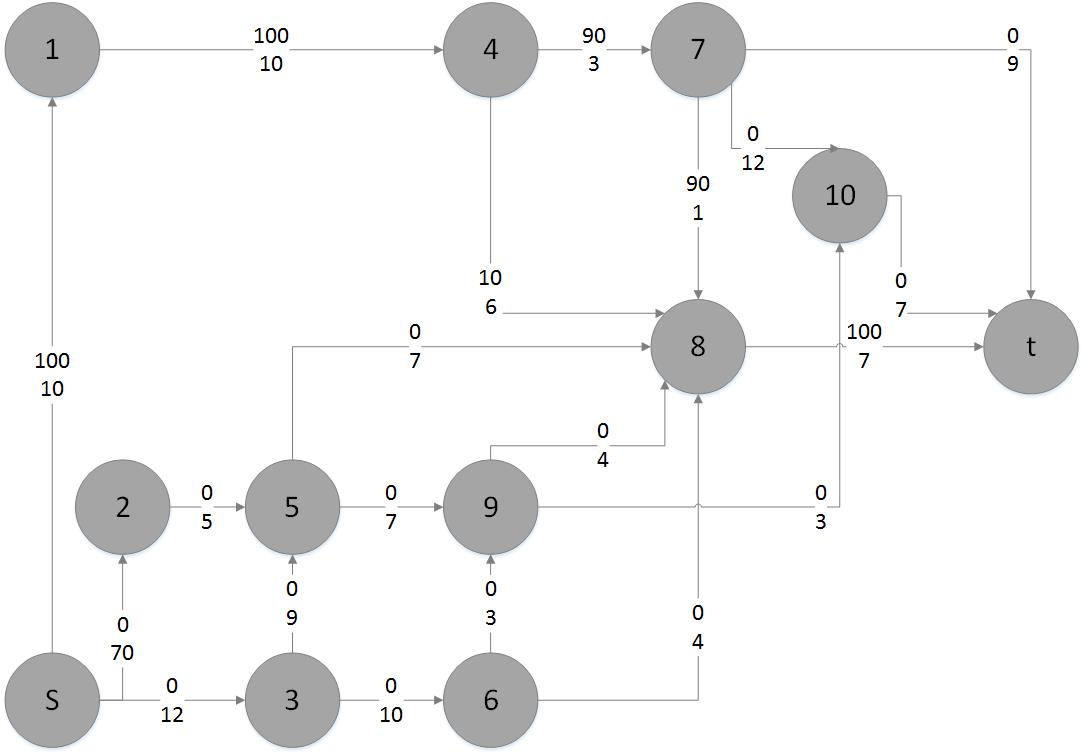
\includegraphics[scale=0.60]{G2_1.jpg}
\caption{Результуюча транспортна мережа}
\end{center}
\end{figure}
\end{center}
Компанія постачальник з'ясувала що передача данних для компанії замовника обійдеться їй в 3120 грошових одиниць.
Тепер постачальник може підготувати комерційну пропозицію для замовника.
%%%%%%%%%%%%%%%%%%%

Задача 3

\indent
Туристичній компанії треба переправити группу відпочиваючих з Одеси до Барселони.Але оскільки группа зібралася дуже піздно, то майже всі квитки на потяг до Києва і літак Київ-Барселона вже розпродані. Компанія зібрала данні про наявні квитки на різні проміжні рейси та потяги і тепер їй треба з'ясувати, як переправити группу відпочиваючих в 100 чоловік найшвидше.

\indent
Зведемо дану задачу до задачі про максимальний потік.
\par Будемо вважати Одесу джерелом $s$ а Барселону - стоком $t$. Авіа та залізничні рейси вважатимемо ребрами мережі, з обмеженнями на пропускну здатність $k(x,y)$ заданої в вигляді таблиці.
\par Час переправи будемо вважати ціною ребра мережі (в хвилинах).
\begin{figure}[h]
\begin{center}
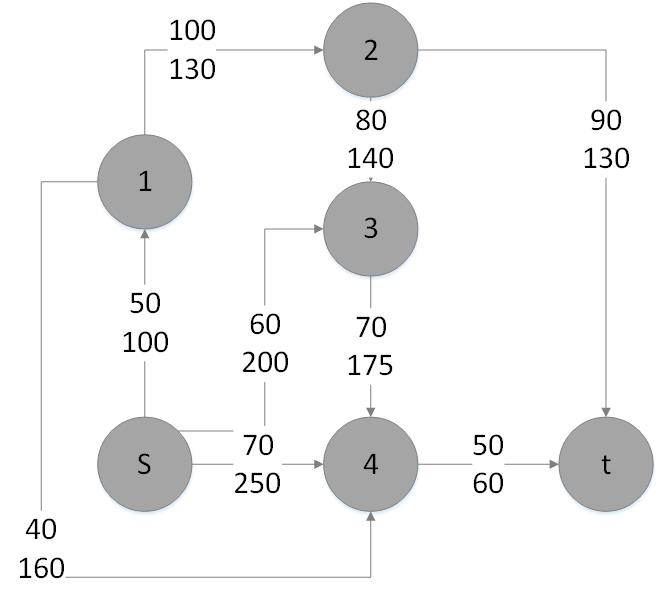
\includegraphics[scale=0.6]{G3.jpg}
\caption{Транспортна мережа}
\end{center}
\end{figure}
\\
\begin{center}
%\begin{turn}{270}
\begin{tabular}{|c|c|c|c|c|c|c|c|c|c|c|c|c|c|c|c|}
\hline
0&50&0&60&70&0     \\ \hline
0&0&100&0&40&0     \\ \hline
0&0&0&80&0&90      \\ \hline
0&0&0&0&70&0       \\ \hline
0&0&0&0&0&50       \\ \hline
0&0&0&0&0&0        \\ \hline
\end{tabular}
%\end{turn}
\end{center}
Час потрібний на переправу заданий матрицею
\begin{center}
\begin{tabular}{|c|c|c|c|c|c|c|c|c|c|c|c|c|c|c|c|}
\hline
0&100&0&200&250&0  \\ \hline
0&0&130&0&160&0    \\ \hline
0&0&0&140&0&130      \\ \hline
0&0&0&0&175&0      \\ \hline
0&0&0&0&0&60       \\ \hline
0&0&0&0&0&0        \\ \hline
\end{tabular}
\end{center}
\indent В результаті роботи програми було отримано наступне рішення:
\begin{center}
\begin{tabular}{|c|c|c|c|c|c|c|c|c|c|c|c|c|c|c|c|}
\hline
0&50&0&0&50&0\\ \hline
0&0&50&0&0&0 \\ \hline
0&0&0&0&0&50 \\ \hline
0&0&0&0&0&0  \\ \hline
0&0&0&0&0&50 \\ \hline
0&0&0&0&0&0  \\ \hline
\end{tabular}
\begin{figure}[h]
\begin{center}
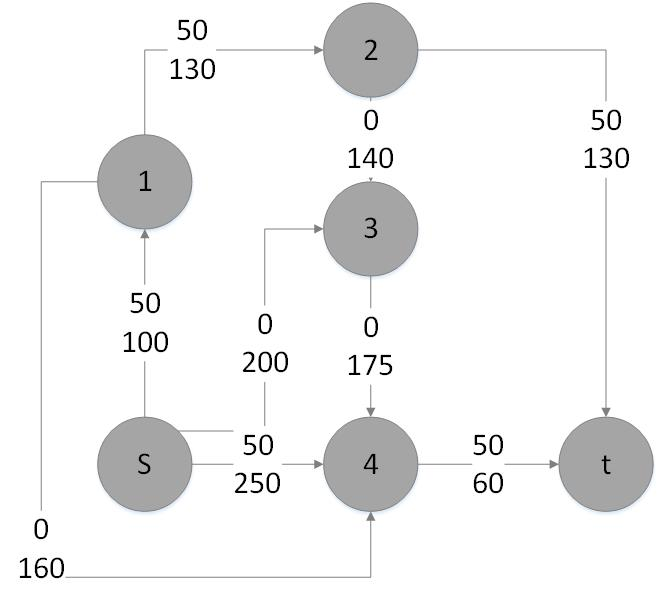
\includegraphics[scale=0.6]{G3_1.jpg}
\caption{Результуюча транспортна мережа}
\end{center}
\end{figure}
\end{center}

В результаті роботи програми компанія знає яким шляхом найкраще доставити туристів до пунктів відпочинку.
%%%%%%%%%%%%%%%%%%%%%%%%%
\newpage
\section{Висновки}
У даній роботі було розглянуто узагальнення задачі про максимальний потік для транспортної мережі з ціною на транспортування одиниці товару через ребро. Як алгоритм рішення був обраний алгоритм Баскера-Гоуєна.Булa розроблена програма на мові с\#, що реалізує даний метод.Робота програми була протестовна на декількох прикладних зaдачaх.
Програмна реалізація вирішує задачу з будь-якою кількістю вершин і ребер.

\newpage
\renewcommand{\bibsection}{\sectioncentered*{Cписок використанної літератури}}
\addcontentsline{toc}{section}{Cписок використанної літератури}

\begin{thebibliography}{99}
\bibitem{ford} Форд, Л.Р. Потоки в сетях. /Л.Р. Форд, Д.Р. Фалкерсон - Москва : Мир, 1966. - 273 с.
\bibitem{taxa} Таха Хемди А. ВВедение в исследование операций /А. Таха - Москва : Вильямс, 2006. - 912 с.
\bibitem{vagner}Вагнер Г. Основы исследования операций. Том 1./Г. Вагнер - Москва : Мир, 1973. - 336 с.
\bibitem{kormen}Кормен Томас Х. Алгоритмы: построение и анализ./К.Х. Томас, Ч.Л. Лейзерсон, Р.Д. Риверс, К. Штайн - Москва : Вільямс, 2005. - 1296 с.
\bibitem{xyt} Ху Т. Целочислнное програмированние и потоки в сетях/Т. Ху - Москва : Мир, 1974. - 513 с.
\bibitem{met} Арсирий А.В. Сетевые модели./ А.В.Арсирій, Б.Ф.Трофимов, Є.М. Страхов - Одеса : Одеський національний університет імені І.І.Мечникова, 2011. - 42 с.
\end{thebibliography}

\sectioncentered*{Додаток A}
\addcontentsline{toc}{section}{Додаток A}
\label{sec:A}

\begin{figure}[h]
\begin{center}
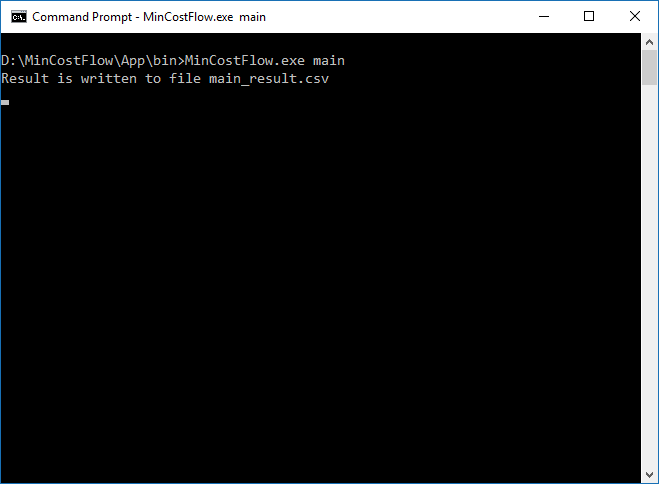
\includegraphics[scale=1]{interface.png}
\caption{Інтерфейс програми}
\end{center}
\end{figure}

\begin{figure}[h]
\begin{center}
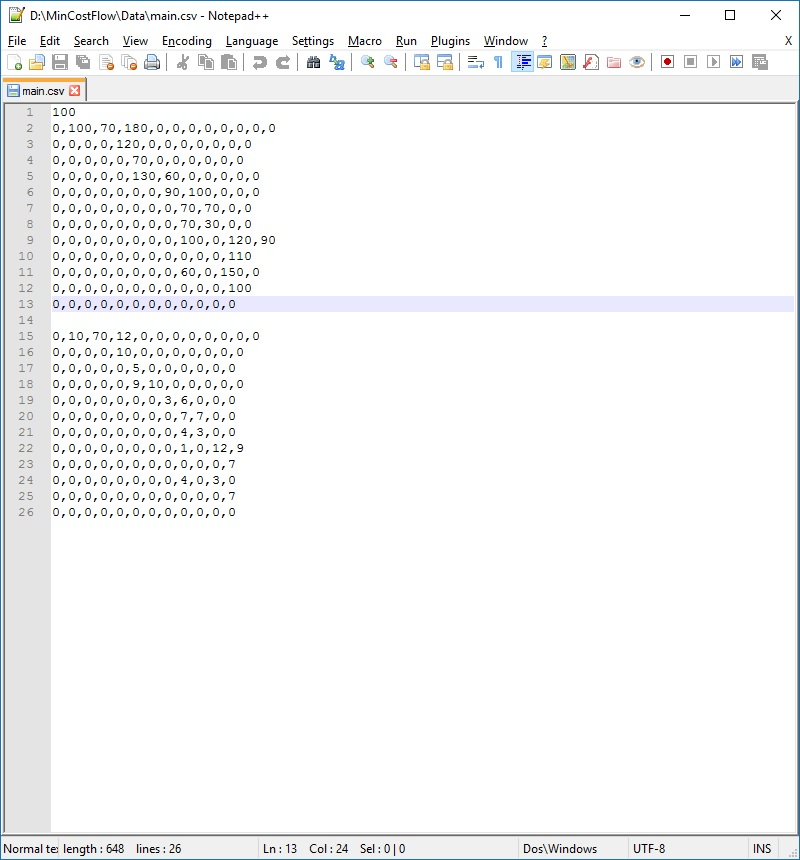
\includegraphics[scale=0.8]{data_in.jpg}
\caption{Формат вхідних данних}
\end{center}
\end{figure}

\begin{figure}[h]
\begin{center}
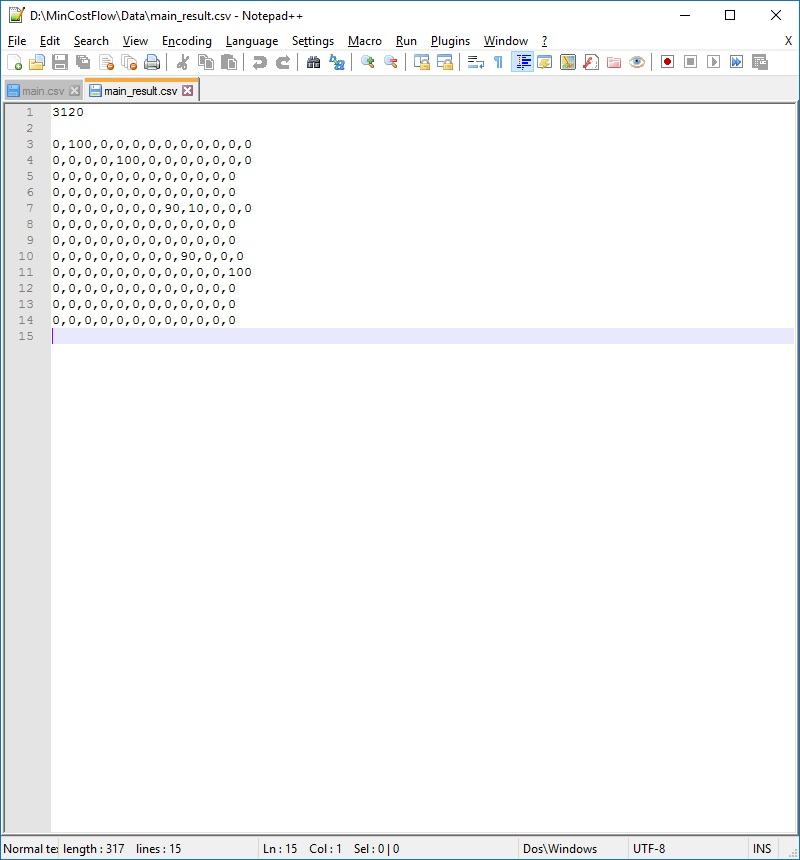
\includegraphics[scale=0.8]{data_out.jpg}
\caption{Формат результату}
\end{center}
\end{figure}

\sectioncentered*{Додаток Б}
\addcontentsline{toc}{section}{Додаток Б}
\label{sec:A}

\begin{lstlisting}[style=csharpinlinestyle]
using System;
using System.Collections;
using System.Collections.Generic;
using System.IO;
using System.Linq;
using System.Text;
using System.Threading.Tasks;

namespace MinCostFlow
{
    class Program
    {
        static void Main(string[] args)
        {
            dataReader data;
            string source = "main";
            try
            {
                if (args.Length > 0)
                {
                    data = getData(args[0]);
                    source = args[0];
                }
                else
                    data = getData(source);
            }
            catch (FileNotFoundException Ex)
            {
                Console.WriteLine($"File {Ex.FileName} was not found, please make sure file is present and has a propper format");
                Console.ReadKey();
                return;
            }
            int[,] flowsCopy = new int[data.flows.GetLength(0), data.flows.GetLength(0)];
            Array.Copy(data.flows, 0, flowsCopy, 0, data.flows.Length);
            FlowCost result = CalculateFlow(data.flows, data.costs, 0, data.flows.GetLength(0) - 1, data.neededFlow);
            var usedFlow = getUsedFlow(flowsCopy, result.resultingFlows);
            writeResult(result.totalCost, usedFlow, source);
            Console.WriteLine($"Result is written to file {source}_result.csv");
            Console.ReadKey();
        }

        private static void writeResult(int totalCost, int[,] usedFlow, string source = "main")
        {
            string fullAppName = System.Reflection.Assembly.GetExecutingAssembly().Location;
            string fullAppPath = System.IO.Path.GetDirectoryName(fullAppName);
            string root = System.IO.Path.GetDirectoryName(fullAppPath);
            root = System.IO.Path.GetDirectoryName(root);
            string DataPath = String.Concat(root, "\\Data", "\\" + source + "_result.csv");

            writeData(DataPath, totalCost, usedFlow);
        }

        private static void writeData(string dataPath, int totalCost, int[,] usedFlow)
        {
            StreamWriter sw = new StreamWriter(dataPath);
            sw.WriteLine(totalCost);
            sw.WriteLine("");
            for (int i = 0; i < usedFlow.GetLength(0); i++)
            {
                var line = "";
                for (int j = 0; j < usedFlow.GetLength(0); j++)
                {
                    line += usedFlow[i, j] + ",";
                }
                line = line.Trim(',');
                sw.WriteLine(line);
            }
            sw.Close();
        }

        private static dataReader getData(string source = "main")
        {
            string fullAppName = System.Reflection.Assembly.GetExecutingAssembly().Location;
            string fullAppPath = System.IO.Path.GetDirectoryName(fullAppName);
            string root = System.IO.Path.GetDirectoryName(fullAppPath);
            root = System.IO.Path.GetDirectoryName(root);
            string DataPath = String.Concat(root, "\\Data", "\\" + source + ".csv");

            if (File.Exists(DataPath))
                return readData(DataPath);
            else
                throw new FileNotFoundException();
        }

        private static dataReader readData(string filePath)
        {
            var result = new dataReader();
            //int[,] flows;
            //int[,] costs;
            try
            {
                StreamReader sr = new StreamReader(filePath);

                string line;

                line = sr.ReadLine();
                result.neededFlow = System.Convert.ToInt32(line.Trim(','));
                line = sr.ReadLine();
                var size = line.Split(',').Length;
                result.flows = new int[size, size];
                result.costs = new int[size, size];
                var lineNum = 0;
                while (line.Length > 2)
                {
                    string[] LimitersStr = line.Split(',');
                    int len = LimitersStr.Length;
                    for (int i = 0; i < size; i++)
                    {
                        result.flows[lineNum, i] = Int32.Parse(LimitersStr[i]);
                    }
                    lineNum++;
                    line = sr.ReadLine();
                }
                lineNum = 0;
                while (sr.Peek() > 0)
                {
                    line = sr.ReadLine();
                    string[] LimitersStr = line.Split(',');
                    //int len = LimitersStr.Length;
                    for (int i = 0; i < size; i++)
                    {
                        result.costs[lineNum, i] = System.Convert.ToInt32(LimitersStr[i]);
                    }
                    lineNum++;
                }
                sr.Close();
                //result.flows = flows;
                //result.costs = costs;
                return result;
            }
            catch (Exception ex)
            {
                return readData("main");
            }
        }

        private static int[,] getUsedFlow(int[,] flows, int[,] resultingFlows)
        {
            var Size = flows.GetLength(0);
            int[,] result = new int[Size, Size];
            for (int i = 0; i < Size; i++)
                for (int j = 0; j < Size; j++)
                {
                    result[i, j] = flows[i, j] - resultingFlows[i, j];
                }
            return result;
        }

        private static FlowCost CalculateFlow(int[,] flows, int[,] costs, int s, int t, int neededFlow)
        {
            var totalFlow = 0;
            var totalCost = 0;
            if (s == t)
                throw new ArgumentException("input and output should be different points");
            MilestoneHist[] path = bfs(flows, costs, s, t);
            while (path[t] != null)
            {
                int maxFlow = getMaxFlowForPath(flows, path, s, t);
                if (neededFlow - totalFlow < maxFlow)
                {
                    maxFlow = neededFlow - totalFlow;
                    flows = updateFlows(maxFlow, flows, path, s, t);
                    totalCost += maxFlow * path[t].totalCost;
                    path = bfs(flows, costs, s, t);
                    totalFlow += maxFlow;
                    return new FlowCost { totalCost = totalCost, resultingFlows = flows, totalFlow = totalFlow };
                }
                flows = updateFlows(maxFlow, flows, path, s, t);
                totalCost += maxFlow * path[t].totalCost;
                path = bfs(flows, costs, s, t);
                totalFlow += maxFlow;
            }
            return new FlowCost { totalCost = totalCost, resultingFlows = flows, totalFlow = totalFlow };
        }

        private static int[,] updateFlows(int maxFlow, int[,] flows, MilestoneHist[] path, int s, int t)
        {
            int to = t;
            int from = path[to].pointNum;
            while (from != -1)
            {
                flows[from, to] -= maxFlow;
                if (flows[from, to] < 0)
                    throw new Exception("result flow can't be less than 0, some error in logic");
                to = from;
                from = path[to].pointNum;
            }
            return flows;
        }

        private static int getMaxFlowForPath(int[,] flows, MilestoneHist[] path, int s, int t)
        {
            int to = t;
            int from = path[to].pointNum;
            var maxFlow = flows[from, to];
            while (from != -1)
            {
                maxFlow = Math.Min(maxFlow, flows[from, to]);
                to = from;
                from = path[to].pointNum;
            }
            return maxFlow;
        }

        public static MilestoneHist[] bfs(int[,] rGraph, int[,] costGraph, int s, int t)
        {
            var debug = 0;
            int Size = rGraph.GetLength(0);
            MilestoneHist[] parent = new MilestoneHist[Size];
            parent[s] = new MilestoneHist { totalCost = 0, pointNum = -1 };
            bool[] visited = new bool[Size];

            Queue q = new Queue();
            q.Enqueue(s);

            while (q.Count != 0)
            {
                int u = (int)q.Dequeue();
                //debug++;
                //if (debug > 10000)
                //    throw new StackOverflowException();

                for (int v = 0; v < Size; v++)
                {
                    if (v != s && rGraph[u, v] > 0 /*&& IsNotCycle(u,v,parent)*/)
                    {
                        if (parent[v] == null)
                        {
                            parent[v] = new MilestoneHist { pointNum = u, totalCost = parent[u].totalCost + costGraph[u, v] };
                            q.Enqueue(v);
                        }
                        else
                        {
                            int newCost = parent[u].totalCost + costGraph[u, v];
                            int oldCost = parent[v].totalCost;
                            if (newCost < oldCost)
                            {
                                parent[v] = new MilestoneHist { pointNum = u, totalCost = newCost };
                                q.Enqueue(v);
                            }
                        }
                    }
                }
            }
            // If we reached sink in BFS starting from source, then return
            // true, else false
            return parent;
        }

        public static Milestone[,] ConvertToMilestones(int[,] costs)
        {
            int size = costs.GetLength(0);
            Milestone[,] res = new Milestone[size, size];
            for (int i = 0; i < size; i++)
                for (int j = 0; j < size; j++)
                {
                    res[i, j] = new Milestone { InitialFlow = costs[i, j], RemainingFlow = costs[i, j] };
                }
            return res;
        }
    }

    class Milestone
    {
        public int InitialFlow { get; set; }
        public int RemainingFlow { get; set; }
        public int Cost { get; set; }
        public Milestone prevMilestone { get; set; }

        public int getTotalCost()
        {
            var maxFlow = this.InitialFlow;
            var totalCost = 0;
            var prevMilestone = this.prevMilestone;
            while (prevMilestone != null)
            {
                maxFlow = Math.Min(maxFlow, prevMilestone.InitialFlow);
                prevMilestone = prevMilestone.prevMilestone;
            }
            prevMilestone = this.prevMilestone;
            while (prevMilestone != null)
            {
                totalCost += prevMilestone.Cost * maxFlow;
                prevMilestone = this.prevMilestone;
            }
            return totalCost;
        }
    }

    class MilestoneHist
    {
        public int pointNum { get; set; }
        public int totalCost { get; set; }

        public static int GetCostByHistory(MilestoneHist[] history)
        {
            throw new NotImplementedException();
        }
    }

    class FlowCost
    {
        public int totalFlow { get; set; }
        public int totalCost { get; set; }
        public int[,] resultingFlows { get; set; }
    }
    class dataReader
    {
        public int neededFlow { get; set; }
        public int[,] flows { get; set; }
        public int[,] costs { get; set; }
    }
}

\end{lstlisting}


\end{document}
